\section{Introduction}
\label{sec:intro}
The problem of equivalence checking between a functional specification and an
implementation written in a low level imperative language such as C
has been of major research interest
and has several important applications such as (a) program verification, where
the equivalence checker is used to verify that the C implementation
behaves according to the specification and (b) translation validation, where
the equivalence checker attempts to generate a proof of equivalence across
the transformations (and translations) performed by an optimizing compiler
and more.

The verification of a C implementation against its manually written
functional specification through manually-coded refinement proofs has been
performed extensively in the seL4 microkernel \cite{seL4}.
Frameworks for program equivalence proofs have been developed in interactive
theorem provers like Coq \cite{programEquivalenceInCoq} where correlations and invariants
are manually identified during proof codification.
On the other hand, programming languages like Dafny \cite{dafny} offer automated program
reasoning for imperative languages with abstract data types such as sets and arrays.
Such languages perform automatic compile-time checks for manually-specified
correctness predicates through SMT solvers.
Additionally, there exists significant prior work on translation validation
\cite{tvi,tristan_tv_eqsat11,stepp_eqsat_llvm11,eqsat,pec,zuck03,zuck05,heffter05,covac,c_to_verilog,kanade09,lopes16,tvoc_cav05,ddec,semalign,oopsla20,tv_oskernel,namjoshi13}
across low level programming languages such as C and assembly.
In most of these applications, soundness in critial,
i.e., if the equivalence checker determines the programs to be equivalent, then the programs are indeed equivalent
and evidently has equivalent observable behaviour. On the other hand, a sound equivalence checker may be incomplete
and fail to prove the programs to be equivalent, even if they were equivalent.

We present \toolName{}, a {\em sound} algorithm to automatically (push-button) search
for a proof of equivalence between a functional specification (written in \SpecL{}) and its
optimized C implementation. We will demonstrate how \toolName{} is capable of
proving equivalence of multiple equivalent C implementations with vastly
different (a) data layouts (e.g. array, linked list representations of a {\em list})
and (b) algorithmic strategies (e.g. alternate algorithms, optimizations) against
a {\em single} functional specification.
This opens the possibility of regression verification \cite{strichman_regressverify,felsing14},
where \toolName{} can be used to automate verification across
software updates that change memory layouts for data structures.

\subsection{Summary}
\label{sec:summary}
We restrict our attention to programs that construct, read, and write
to recursive data structures. In languages like C, pointer and array based
implementations of these data-structures are prone to safety and liveness bugs.
Similar recursive data structures are also available in safer functional languages like Haskell,
where algebraic data types (ADTs) \cite{hope} ensure several safety properties.
We define a minimal functional language, called \SpecL{}, that enables the safe
and succinct specification of programs manipulating and traversing recursive data structures.
\SpecL{} is equipped with ADTs as well as boolean and bitvector (\type{i<N>}) types.

Next, we give a brief overview of our approach through an example.
This allows us to introduce the major subgoals and
we state our primary contributions in the next section.

\begin{figure}
\begin{tabular}{@{}c@{}c@{}}
\begin{subfigure}[b]{\textwidth}
\begin{center}
\begin{allLangEnvFoot}
~{\scriptsize \textcolor{mygray}{A0:}}~ type List = LNil | LCons (val:i32, tail:List).
~{\scriptsize \textcolor{mygray}{A1:}}~
~{\scriptsize \textcolor{mygray}{A2:}}~ fn mk_list_impl (n:i32) (i:i32) (l:List) : List =
~{\scriptsize \textcolor{mygray}{A3:}}~    if ${\tt i \geq_u n}$ then l
~{\scriptsize \textcolor{mygray}{A4:}}~             else make_list_impl(n, i+${\tt 1_{i32}}$, LCons(i, l)).
~{\scriptsize \textcolor{mygray}{A5:}}~
~{\scriptsize \textcolor{mygray}{A6:}}~ fn mk_list (n:i32) : List = mk_list_impl(n, ${\tt 0_{i32}}$, LNil).
\end{allLangEnvFoot}
\end{center}
\caption{\label{fig:llAllocSpec}Spec program}
\end{subfigure}%
\\
\begin{subfigure}[b]{\textwidth}
\begin{center}
\begin{allLangEnvFoot}
~{\scriptsize \textcolor{mygray}{B0: }}~ typedef struct lnode {
~{\scriptsize \textcolor{mygray}{B1: }}~   unsigned val; struct lnode* next;
~{\scriptsize \textcolor{mygray}{B2: }}~ } lnode;
~{\scriptsize \textcolor{mygray}{B3: }}~ 
~{\scriptsize \textcolor{mygray}{B4: }}~ lnode* mk_list(unsigned n) {
~{\scriptsize \textcolor{mygray}{B5: }}~   lnode* l = NULL;
~{\scriptsize \textcolor{mygray}{B6: }}~   for (unsigned i = 0; i < n; ++i) {
~{\scriptsize \textcolor{mygray}{B7: }}~     lnode* p = malloc(sizeof lnode);
~{\scriptsize \textcolor{mygray}{B8: }}~     p$\rightarrow$val = i; p$\rightarrow$next = l; l = p;
~{\scriptsize \textcolor{mygray}{B9: }}~   }
~{\scriptsize \textcolor{mygray}{B10:}}~   return l;
~{\scriptsize \textcolor{mygray}{B11:}}~ }
\end{allLangEnvFoot}
\end{center}
\caption{\label{fig:llAllocC}C program with {\tt malloc()}}
\end{subfigure}%
\\
\end{tabular}
\caption{\label{fig:llAllocSpecAndC}Spec and C programs each constructing a Linked List.}
\end{figure}


\begin{figure}[H]
\begin{tabular}{cc}
\begin{subfigure}[b]{0.37\textwidth}
\begin{center}
\begin{allLangEnvFoot}
~{\scriptsize \textcolor{mygray}{S0:}}~ List mk_list (i32 n) {
~{\scriptsize \textcolor{mygray}{S1:}}~   List l $\coloneqq$ LNil;
~{\scriptsize \textcolor{mygray}{S2:}}~   i32  i $\coloneqq$ ${\tt 0_{i32}}$;
~{\scriptsize \textcolor{mygray}{S3:}}~   while ${\tt \neg (i \geq_{u} n)}$:
~{\scriptsize \textcolor{mygray}{S4:}}~     l $\coloneqq$ LCons(i, l);
~{\scriptsize \textcolor{mygray}{S5:}}~     i $\coloneqq$ i + ${\tt 1_{i32}}$;
~{\scriptsize \textcolor{mygray}{S6:}}~   return l;
~{\scriptsize \textcolor{mygray}{SE:}}~ }
\end{allLangEnvFoot}
\vspace{35px}
\end{center}
\caption{\label{fig:llAllocSpecIR}(Abstracted) Spec IR}
\end{subfigure}%
&
\begin{subfigure}[b]{0.63\textwidth}
\begin{center}
\begin{allLangEnvFoot}
~{\scriptsize \textcolor{mygray}{C0:}}~ i32 mk_list (i32 n) {
~{\scriptsize \textcolor{mygray}{C1:}}~   i32 l $\coloneqq$ ${\tt 0_{i32}}$;
~{\scriptsize \textcolor{mygray}{C2:}}~   i32 i $\coloneqq$ ${\tt 0_{i32}}$;
~{\scriptsize \textcolor{mygray}{C3:}}~   while ${\tt i <_{u} n}$:
~{\scriptsize \textcolor{mygray}{C4:}}~     i32 p $\coloneqq$ malloc$_{\tt C4}$(sizeof(lnode));
~{\scriptsize \textcolor{mygray}{C5:}}~     $\mem{}$ $\coloneqq$ $\mem{}$[p+offsetof(lnode,val)$\leftarrow$i]$_\type{i32}$;
~{\scriptsize \textcolor{mygray}{C6:}}~     $\mem{}$ $\coloneqq$ $\mem{}$[p+offsetof(lnode,next)$\leftarrow$l]$_\type{i32}$;
~{\scriptsize \textcolor{mygray}{C7:}}~     l $\coloneqq$ p;
~{\scriptsize \textcolor{mygray}{C8:}}~     i $\coloneqq$ i + ${\tt 1_{i32}}$;
~{\scriptsize \textcolor{mygray}{C9:}}~   return l;
~{\scriptsize \textcolor{mygray}{CE:}}~ }
\end{allLangEnvFoot}
\end{center}
\caption{\label{fig:llAllocCIR}(Abstracted) C IR}
\end{subfigure}%
\\
\end{tabular}
\caption{\label{fig:llAllocSpecIRAndCIR}IRs for the \SpecL{} and C Programs in \cref{fig:llAllocSpec,fig:llAllocC} respectively.}
\end{figure}


\Cref{fig:llAllocSpec,fig:llAllocC} show the construction of lists in \SpecL{} and C respectively.
The \type{List} ADT in the \SpecL{} program in defined at line {\tt A0} in \cref{fig:llAllocSpec}.
An empty \type{List} is represented by the constructor \cons{LNil}, where as a non-empty list uses
the \cons{LCons} constructor to combine its first value ({\tt val}\ctype{i32}) and
the remaining list ({\tt tail}\ctype{List}).
The inputs to a \SpecL{} procedure are its well-typed arguments, which may include recursive data structure
values. The inputs to a C procedure are its explicit arguments and the implicit state of program memory
at procedure entry.
We lower both \SpecL{} and C programs to a common intermediate representation (IR)
as shown in \cref{fig:llAllocSpecIR,fig:llAllocCIR}.
For the \SpecL{} program in \cref{fig:llAllocSpec},
the tail-recursive function {\tt mk\_list\_impl} is converted to a loop and
inlined in the top-level function {\tt mk\_list}.
For the C program in \cref{fig:llAllocC},
the sizes and memory layouts of both scalar (e.g., \type{unsigned})
and compound (e.g., \type{struct lnode}) types are concretized in the IR.

\begin{figure}
\begin{tabular}{@{}c@{}c@{}}
\begin{subfigure}[b]{0.5\textwidth}
\begin{center}
{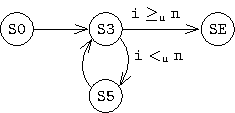
\includegraphics[scale=1.4]{chapters/figures/figMallocSpecCfg.pdf}}
\vspace{15pt}
\end{center}
\caption{\label{fig:llAllocSpecIRCFG}CFG of \SpecL{} program}
\end{subfigure}%
&
\begin{subfigure}[b]{0.5\textwidth}
\begin{center}
{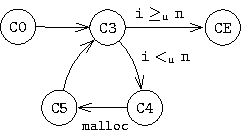
\includegraphics[scale=1.4]{chapters/figures/figMallocCCfg.pdf}}
\end{center}
\caption{\label{fig:llAllocCCFG}CFG of C program}
\end{subfigure}%
\\
\end{tabular}
\caption{\label{fig:mallocSpecCFGAndCCFG}CFG representation of Spec and C IRs shown in \cref{fig:llAllocSpecIR,fig:llAllocCIR} for the {\tt mk\_list} procedures in \cref{fig:llAllocSpec,fig:llAllocC} respectively.}
\end{figure}


\Cref{fig:llAllocSpecIRCFG,fig:llAllocCCFG} show the Control-Flow Graph (CFG) representation
of the \SpecL{} and C IR programs in \cref{fig:llAllocSpecIR,fig:llAllocCIR} respectively.
Each node represent a PC location of its corresponding program, and each edge represent
conditional transition between PCs through instruction execution.
For brevity, we often represent a sequence of instructions with a single edge, e.g.,
in \cref{fig:llAllocCCFG}, the edge \cpath{5,3} represents the path \cpath{5,6,7,8,3}.

\begin{figure}[H]
\begin{tabular}{cc}
\begin{subfigure}[b]{1\textwidth}
\begin{center}
{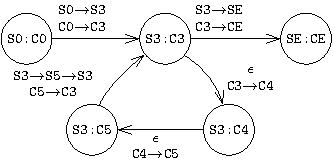
\includegraphics[scale=1.2]{chapters/figures/figMallocProductCfg.pdf}}
\end{center}
\end{subfigure}%
\end{tabular}
\caption{\label{fig:llAllocProductCFG}Product-CFG between \cref{fig:llAllocSpecIRCFG,fig:llAllocCCFG}}
\end{figure}


We construct a {\em bisimulation relation} to identify equivalence between the two programs.
A bisimulation relation correlates the transitions of \SpecL{} and C programs in lockstep, such that the
lockstep execution ensures identical observable behavior.
A bisimulation relation between two programs can be represented using a {\em product program}
\cite{covac} and the CFG representation of a product program is called a {\em product-CFG}.
\Cref{fig:llAllocProductCFG} shows a product-CFG, that encodes the lockstep execution
(bisimulation relation) between the CFGs in \cref{fig:llAllocSpecIRCFG,fig:llAllocCCFG}.

\begin{table}[H]
\begin{center}
\caption{\label{tab:llproductInv}Node Invariants for Product-CFG in \cref{fig:llAllocProductCFG}}
\setlength{\belowcaptionskip}{-30pt}
\begin{footnotesize}
\begin{tabular}{|c|llll|}
\hline
\tt PC-Pair & \multicolumn{4}{c|} {\tt Invariants} \\
\hline
\hline
${\tt (S0:C0)}$ &
\multicolumn{4}{l|} {\Tstrut ${\tt { \circled{P}}\  n_{S}=n_{C}}$} \\
${\tt (S3:C3)}$ &
\Tstrut  ${\tt {\scriptsize \circled{I1}}\  n_{S}=n_{C}}$ & ${\tt {\scriptsize \circled{I2}}\  i_{S}=i_{C}}$ & ${\tt {\scriptsize \circled{I3}}\  i_{S} \leq_{u} n_{S}}$ & ${\tt {\scriptsize \circled{I4}}\  l_{S}\indEq{}Clist^{lnode}_{m}(l_{C})}$ \\
${\tt (S3:C4)\ (S3:C5)}$ &
\Tstrut  ${\tt {\scriptsize \circled{I5}}\  n_{S}=n_{C}}$ & ${\tt {\scriptsize \circled{I6}}\  i_{S}=i_{C}}$ & ${\tt {\scriptsize \circled{I7}}\  i_{S} <_{u} n_{S}}$ & ${\tt {\scriptsize \circled{I8}}\  l_{S}\indEq{}Clist^{lnode}_{m}(l_{C})}$ \\
${\tt (SE:CE)}$ &
\multicolumn{4}{l|} {\Tstrut  ${\tt {\circled{E}}\  ret_{S}\indEq{}Clist^{lnode}_{m}(ret_{C})}$} \\
\hline
\end{tabular}
\end{footnotesize}
\end{center}
\end{table}


At each node of the product-CFG, invariants relate the states of the \SpecL{} and C program respectively.
\Cref{tab:llproductInv} lists invariants for the product-CFG in \cref{fig:llAllocProductCFG}.
At the start node \scpc{0}{0} of the product-CFG, the precondition $Pre$ (labeled \circled{\small P})
ensures equality of input arguments \sv{n} and \cv{n} at the programs' entry.
Inductive invariants (labeled \circled{\small I}) are inferred at
each intermediate product-CFG node (e.g., \scpc{3}{3}) relating both programs' states.
For example, at node \scpc{3}{5}, \circled{\small I6} $\sv{i} = \cv{i}$ is an inductive invariant.

In \cref{tab:llproductInv}, the invariant \circled{\small I4} $\sv{l} \indEq{} \lifted{list}{\mem{}}{lnode}{\cv{l}}$
is an example of a \recursiveRelation{} and represents equality between the \SpecL{} \type{List} variable \sv{l}
and the \type{{List}} represented by chasing the \type{lnode} pointers starting at \cv{l}.
\lift{list}{\mem{}}{lnode} is an example of a {\em lifting constructor} that `lifts' a C pointer value
(pointing to an object of type \type{struct lnode}) and the C memory state \mem{}
to a \SpecL{} \type{List} value, and is defined as follows:
\begin{equation}
\label{eqn:clist}
\begin{split}
U_C:\ &\lifted{list}{\mem{}}{lnode}{p \ctype{i32}} = \sumIf{p=0} \ \sumThen{\cons{LNil}} \\ & \qquad\qquad\ \ \ \sumElse{\cons{LCons}(\structPointer{p}{\mem{}}{lnode}{val}, \lifted{list}{\mem{}}{lnode}{\structPointer{p}{\mem{}}{lnode}{next}})}
\end{split}
\end{equation}

Product-CFG invariants involving \recursiveRelations{} (e.g., \circled{\small I4}) allow
us to express equality between native \SpecL{} values with the C program state.
Assuming that the precondition $Pre$ (\circled{\small P}) holds at the entry node \scpc{0}{0},
a bisimulation check involves checking that the inductive invariants hold too,
and consequently the postcondition $Post$ (\circled{\small E}) holds at the exit node \scpc{E}{E}.
Checking whether an invariant holds results in proof queries.
These proof obligations are expressed as relational Hoare triples \cite{relationalHoareLogic,hoareTriple}
and discharged through a proof discharge algorithm i.e. a solver.
We give a more formal exposition of the concepts introduced in this summary in the coming chapters.

\subsection{Our Contributions}
\label{sec:contribs}
As previously summarized in \cref{sec:summary}, showing equivalence of a \SpecL{} and a C program
through a bisimulation proof requires three major procedures:
\circled{\small 1} An algorithm for construction of a product-CFG by correlating program executions
across the \SpecL{} and C programs respectively.
\circled{\small 2} An algorithm for identification of inductive invariants at intermediate correlated PCs.
\circled{\small 3} An algorithm for solving proof obligations containing \recursiveRelations{}.
Our major contributions are as follows:

\begin{itemize}
\item Proof Discharge Algorithm: Solving proof obligations (\circled{\small 3})
involving \recursiveRelations{} is rather interesting and forms our primary contribution.
We describe a {\em sound} proof discharge algorithm capable of tackling proof obligations involving
\recursiveRelations{} using off-the-shelf SMT solvers. Our proof discharge algorithm is also capable of
reconstruction of counterexamples for the original proof query from models returned by the individual SMT queries.
These counterexamples are the backbone of counterexample-guided algorithms for
\circled{\small 1} and \circled{\small 2} steps. As part of our proof discharge procedure,
we reformulate equality of values (i.e. \recursiveRelations{}) as equivalence of their corresponding programs
and discharge these proof queries using a nested (albeit much simpler) bisimulation check.

\item Spec-to-C Automatic Equivalence Checker Tool: Our second contribution is \toolName{}, an equivalence checker tool
capable of proving equivalence between a \SpecL{} and a C program automatically.
\toolName{} is based on
the Counter tool\cite{oopsla20} and uses modified versions of (a) counterexample-guided correlation algorithm for
incremental construction of a product-CFG and (b) counterexample-guided invariant inference algorithm
for inference of inductive invariants at correlated PCs in the (partially constructed) product-CFG.
\toolName{} discharges required verification conditions (i.e. proof obligations) using our Proof Discharge Algorithm.
\Cref{fig:diagram} gives an overview of the complete algorithm.
\end{itemize}

\begin{figure}
\begin{center}
{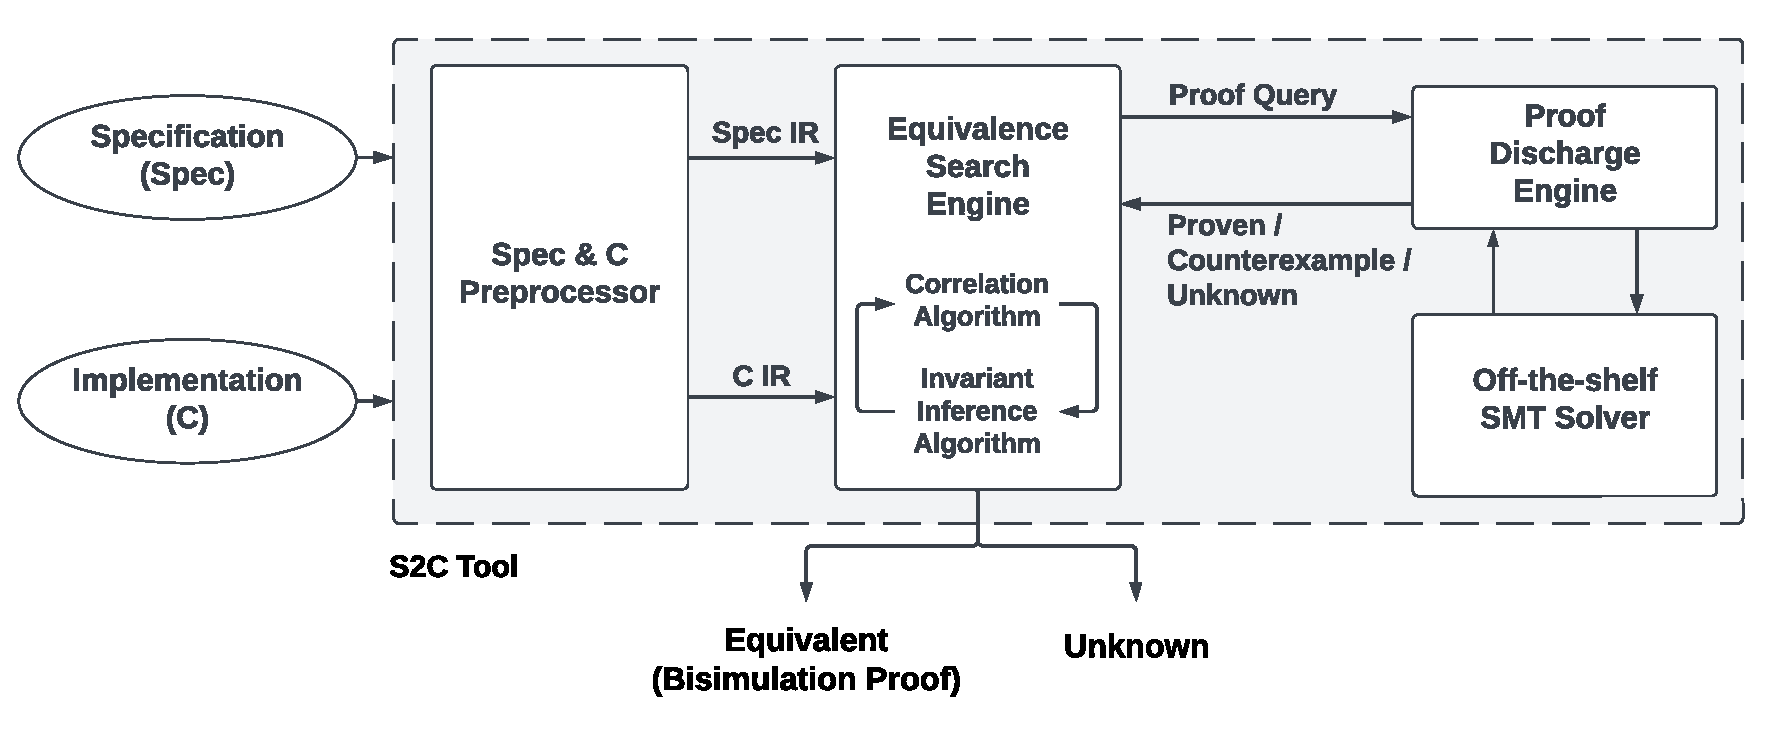
\includegraphics[scale=0.495]{chapters/figures/figDiagram.pdf}}
\end{center}
\caption{\label{fig:diagram}Overview of our equivalence checker algorithm \toolName{}.
The inputs to \toolName{} are the \SpecL{} and C programs.
\toolName{} either successfully finds a bisimulation proof implying equivalence or
soundly returns an unknown verdict.}
\end{figure}